\chapter{Casing}

% Another point to note is, that the casing was build with modularity in mind. This enables to repair 
It might seem like the casing is not very significant, even though the design and function of all kinds of device's exteriors is crucial. The simplest of casings often have multiple design stages and variations with different advantages. Since the Tesla coil is intended as a consumer product, the casing plays an important role for its appearance. But apart from optics, there are a lot of safety hazards, which the casing has to account for. Most notably is the very real fire risk, which goes along playing with open plasma.


\section{Concept design}
\label{sec:concept-design}

There are four main parts that are essential to consider while constructing the Tesla coil - the primary coil, the secondary coil, the \gls{pcb}, and the top electrode. Technically, those can be placed in any way possible, but there is a reasonable standard practice for their placement, especially for the coils and the top electrode. 

\begin{marginfigure}[1cm]
    \centering
    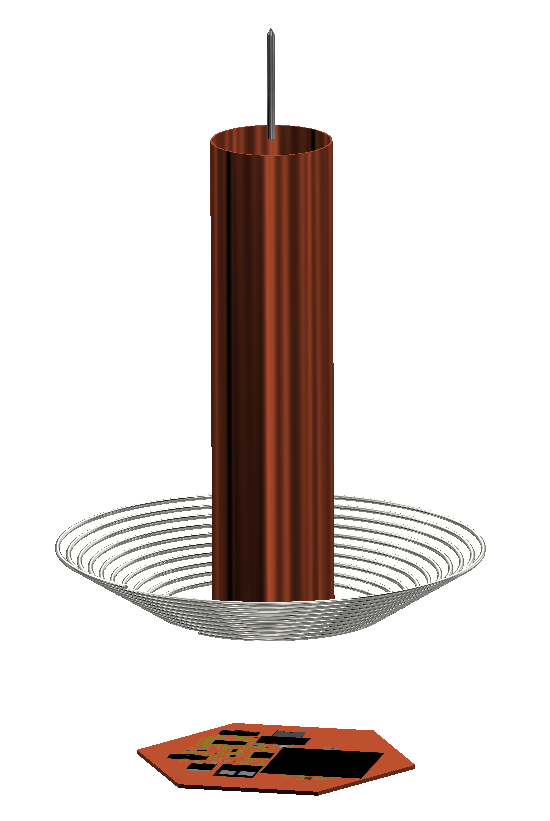
\includegraphics[width=1.2\textwidth]{kassandra/resources/JerJerWoBistDuKonzept.PNG}
    \caption{Concept design}
    \label{fig:envision}
\end{marginfigure}

As seen in figure \ref{fig:envision}, the secondary coil is perpendicular, and the primary coil is angled at 30° to the horizontal, the primary coil design choices have already been detailed in the previous part at the end of section \ref{sec:designing-the-primary}. This is the easiest way to calculate and also the most practical way to design the secondary. The end of the secondary could technically be used as the top electrode, but the copper will definitively melt as soon as it emits a spark. So it has to be out of a high temperature resistant material that is also conductive. The placement for the top electrode seems very obvious, but there is an explanation. If the arching point of the electrode is placed further away from the secondary, the behavior of the coils will become less predictable the more distance is between them. So the most practical placement is in the middle and a few centimeters above the secondary coil.

Technically the \gls{pcb} can be placed anywhere\sidenote{There should be a reasonable distance between the PCB and the coils to ensure that the electrical field does not interfere with the circuitry.}as long as it can be connected to the coils. However, to make transportation the easiest, the casing for the \gls{pcb} should be right beneath the coils. This way, everything needed stays in one place. 

\section{Materials}

Deciding which materials to use is also a tedious task because there are a lot of details and possibilities that have to be considered when designing a Tesla coil. Many factors determine the best working material, most affecting the coils directly and therefore being unsuitable, but others are scrapped because of their low availability or costly construction.

\subsection{Metals}
\label{subsec:materials-metals}

Metal is a popular choice for building high-grade casings because of its low price and good machinability. However, metals are rather unsuitable for a Tesla coil, mainly because of their electrical conductivity, which would pose an unnecessary safety risk to the user when touched. On one side, because some internal connection error could in the worst case be lethal, but also because if not properly grounded, static electricity could build up in the casing and shock everyone touching it. Another critical factor is that metals have very high permeability, weakening any magnetic field. This would not be a big problem for the \gls{pcb} enclosure but would certainly cause issues when used for the support of the primary or secondary coil.

\subsection{Woods}

One material that is not often used for casings, especially for commercial products, is wood, mainly because it is more expensive and harder to work with than metal. This Tesla coil is not like any device, but wood is still not a good option, most notably because the top electrode emits a high-temperature spark which could inflame the wooden casing. Making the casing for only the \gls{pcb} wooden would not work either because if the capacitance of the secondary coil changes, the driver operates outside of its ideal conditions and dissipates a lot of energy as heat, potentially inflaming the wood.

\subsection{Glass}

Glass is an electrical insulator, so it would not interfere with the magnetic field, has very high-temperature resistance, and has a polished look. It also comes in various opacities, and surface finishes making the casing very customizable. The main disadvantage of glass is its high production costs. Due to the Tesla coil not being commercially produced, this kind of casing would be unsustainable.

\subsection{Plastics}

\glsunset{pvcp}\glsunset{pmma}\glsunset{pvcu}\glsunset{ptfe}
The only remaining option for the type of casings material would be plastic. However, plastic is not plastic. The two types of plastic with the highest availability, in this case, would be \gls{pvcp} and \gls{pmma}\sidenote{also commercially known as acrylic glass or plexiglass}. There is also \gls{pvcu}, but given that it is harder to process and also less available, \gls{pvcp} is preferred. \gls{pvcp} would be a lot better than \gls{pmma} when it comes to cost and availability, but it cannot provide the suitable characteristics for the Tesla coil. One problem with \gls{pvcp} is its water absorption because due to water's diamagnetic properties, it heats up in an oscillating magnetic field, i.e., it is wasting energy. \gls{pvcp}s water absorption over 24 hours lies at a maximum of 1\% of its total weight. \gls{pmma}, in comparison, has an absorption of 0.4\% at max. On the other hand, \gls{pvcu} has an even more ideal water absorption at 0.1\%. \sidecite{water-absorption} The casing should not be out of \gls{pvcp} or \gls{pvcu} because of its poor temperature resistance, which starts to deform at around 60°C, while \gls{pmma} only starts at about 100°C. \gls{pmma} is not ideal in any way, but due to its easy availability and better properties, it was chosen for the casing. 

The most ideal plastic would be \gls{ptfe}\sidenote{also commercially known as Teflon}, which has a maximum of 0.01\% water absorption, a tenth better than \gls{pvcu}. The temperature resistance is also better than \gls{pmma} because it can be used at a working temperature of 280°C\sidecite{blue-bible}. But \gls{ptfe} was not used as a casing because it was unavailable, but it might be considered in a future build.  

\subsection{Conclusion}

In figure \ref{fig:material-score}, all previously discussed materials are given a subjective score from 1 to 10 in the four most important categories. The score in the circle is then determined by the average points of these categories, visualizing which material is best suited for the Tesla coil. Both \gls{ptfe} and \gls{pmma} have the same total score, but as already mentioned above, \gls{ptfe} wasn't used because of the low availability.  

\begin{figure}[h!]
    \centering
    \begin{tabular}{cc}
      \materialscore{Metal}{4}{1}{8}{6}{3} & \materialscore{Wood}{5}{6}{2}{7}{6} \\
      \materialscore{Glass}{7}{9}{9}{1}{10} & \materialscore{PMMA}{8}{8}{6}{9}{7} \\
      \materialscore{PVC-U}{7}{9}{6}{9}{5} & \materialscore{PTFE}{8}{10}{7}{8}{6} \\
      \multicolumn{2}{l}{
      \begin{tabular}{cl}
        \\
        {\color{gr70}\faIcon{magnet}} &  Magnetic and Electrical Properties \\
        {\color{gr70}\faIcon{fire}} &  Temperature resistance \\
        {\color{gr70}\faIcon{euro-sign}} &  Machinability and cost \\
        {\color{gr70}\faIcon{eye}} &  Optics
      \end{tabular}}
    \end{tabular}
    \caption{Bottom text}
    \label{fig:material-score}
\end{figure}



\section{Structure for the Coils}

As mentioned in section \ref{sec:concept-design}, both coils have a fixed position and shape, but to ensure this, the casing has to be built based on them. The secondary is easy to support, but the primary has a unique shape that has to be kept in form. 

\subsection{Primary Coil}

The primary coil's holding structure consists of six supports arranged in a hexagonal way. Every support is a triangular-shaped slope with an angle of 30°, on top of which the primary coil rests. In order to keep the primary coil in place, small half-circles have been cut out for every turn. However, to keep the coil's shape, the ten slots on each support have to be shifted up by one-sixth of the distance between each other.

\begin{figure}[h!]
    \centering
    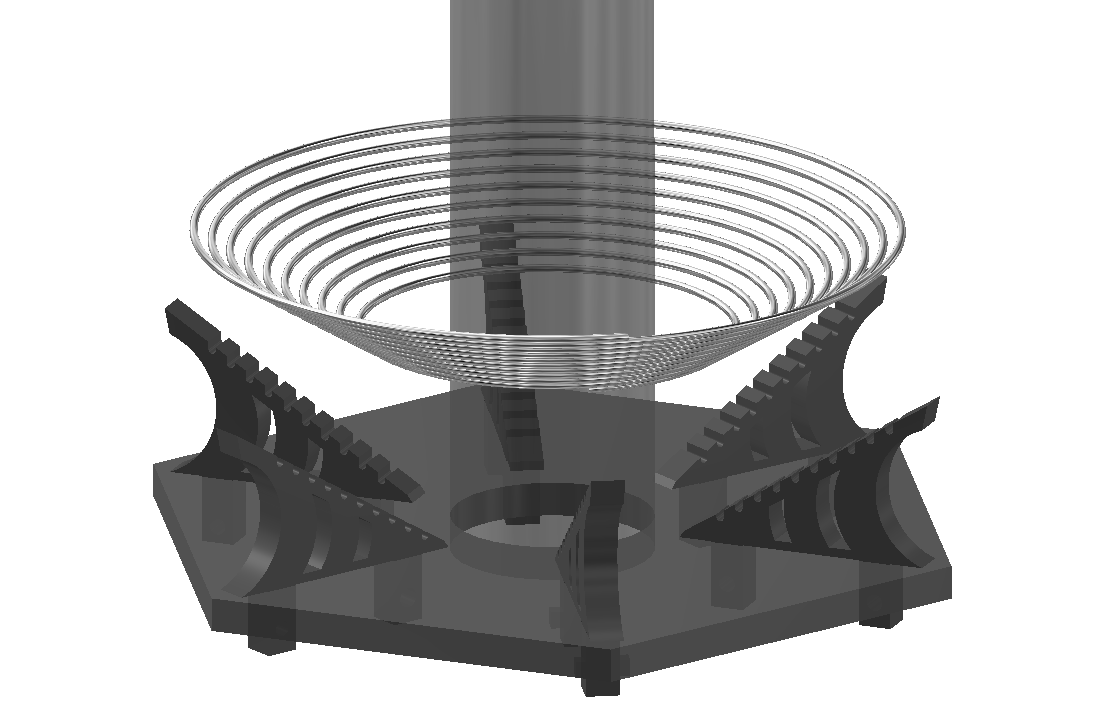
\includegraphics[width=1\textwidth]{kassandra/resources/endeMeinerHoffnung.png}
    \caption{3D view of the primary supports}
    \label{fig:primary-supports}
\end{figure}

To avoid gluing the supports to the base plate, a bolt was used to keep it in place, as shown in figure \ref{fig:stayer}. This mechanism was mainly designed for testing purposes as it is easier to assemble and disassemble. In a possible future version or commercial release, it would be safer if the supports were glued on. Also, as shown, the supports have a unique design. This was mostly done to make them look elegant and not stand out too much. That makes them lighter, but given that the supports are just a tiny fraction of the Tesla coil's weight, it does not make much of a difference.

\begin{figure}[h!]
    \begin{subfigure}{0.5\textwidth}
        \centering
        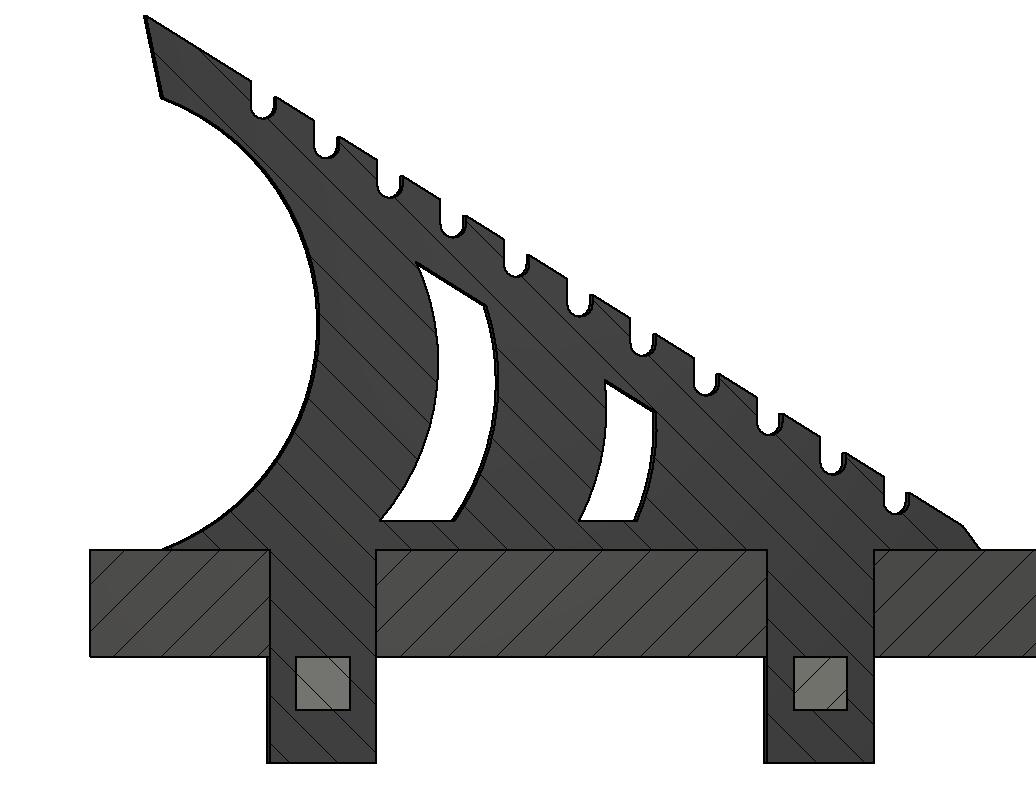
\includegraphics[width=\textwidth]{kassandra/resources/endeMeinerHoffnungInSemi2DStayer.PNG}
    \end{subfigure}%
    \begin{subfigure}{0.5\textwidth}
        \centering
        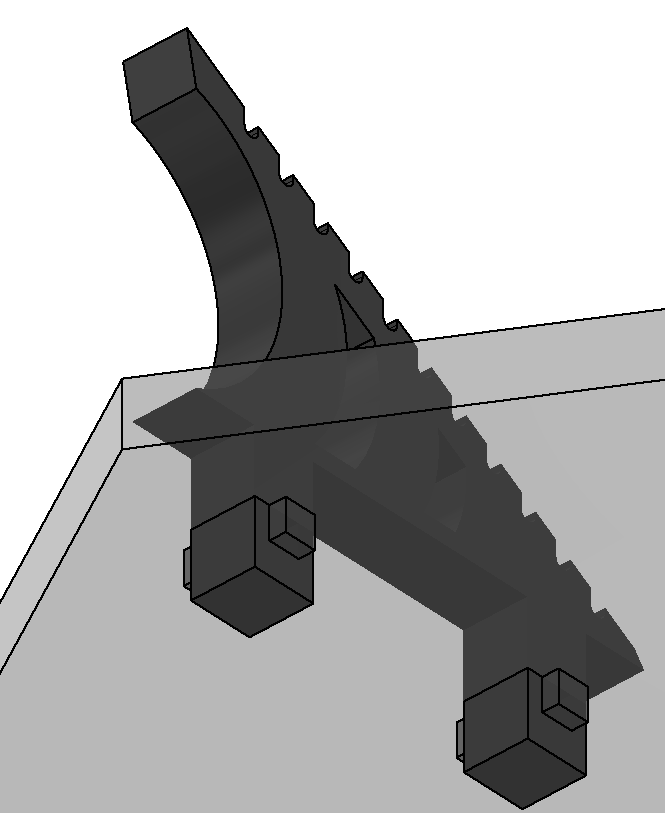
\includegraphics[width=0.7\textwidth]{kassandra/resources/endeMeinerHoffnungIn3DStayer.PNG}
    \end{subfigure}
    \centering
    \caption{Fastening of the supports}
    \label{fig:stayer}
\end{figure}

\subsubsection{Manufacturing}

Complex structures like the primary supports, that on top of that are also small are best manufactured with an automated process like 3D printing. This way makes it possible to constructed both the supports and the platform their mounted on in one piece, erasing the need for bolts entirely. But the way 3D printing works by drawing multiple layers of fine plastic lines makes the end product inaccurate. Which is unsuitable for the small half circles on the supports, as they will most likely end up too small for the wire of the primary coil. 

\subsection{Secondary Coil}

The core of the secondary coil was one of the easier parts to design because it essentially just consists of a \(30\,mm\) \gls{pmma} tube with a thickness of 3mm and a length of \(120\,mm\). A few millimeters from the top of the tube, a small hole was drilled to guide the wire to the inside and connect it to the top electrode. The 330 turns of \(0.35\,mm\) wire were then wound by hand and then coated with protective and insulating varnish to prevent the wire from loosening and cross-arcing to occur.

\section{Primary Wire Bending}

After the supports for the primary coil have been designed, the the coils itself still has to be bent. Simply bending the wire by placing it in the slots one after another is not an option, because it takes a considerable amount of force to hold a tensioned \(1.2\,mm\) wire in place\sidenote{This force could be brought up by glue, but that would be very unprofessional}. 
This force is due to the elastic component of the wire's deformation, which tries to bend the wire back to its original shape. 

\subsection{Springtrap}

To remove this component, the wire has to be overbend by a specific angle and to a specific radius. Those values are determined by the springback factor \(k_s\)\sidecite{blue-bible}, and the desired angle and radius, which remain due to purely plastic deformation. \(k_s\) highly depends on the material and geometry, and usually can be found in large databases.

However, since those are often not freely available\sidenote{Especially not for silver-coated copper wires}, this factor had to be measured by hand. This was done by bending the wire by a specific angle \(\alpha_1\) and measuring the angle \(\alpha_2\) that it sprung back to. Because \(k_s\) is geometry-dependent, this measurement had to be repeated for multiple diameters. \(k_s\) then simply is the ratio between \(\alpha_2\) and \(\alpha_1\). Figure \ref{fig:springback} shows these calculated values as well as their linear regression fit.

\begin{marginfigure}[-1cm]
    \centering
    \resizebox{0.98\textwidth}{!}{
    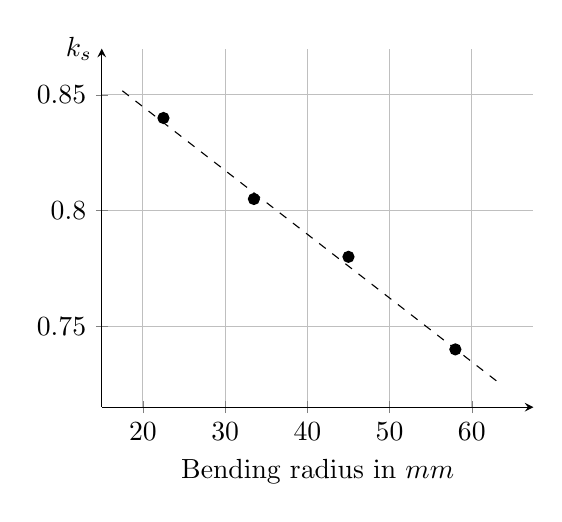
\begin{tikzpicture}
      \begin{axis}[
        xlabel=Bending radius in \(mm\),
        ylabel=\(k_s\),
        y label style={at={(axis description cs:0,1)},rotate=-90},
        grid=major,
        axis lines=left,
        ymin = 0.715,
        ymax = 0.87,
        xmin = 15,
        xmax = 67.5,
        scale = 0.8
        ]
        \addplot[only marks] coordinates{(22.5,0.84)(33.5,0.805)(45,0.78)(58,0.74)};
        \addplot[domain=17.5:63.5, dashed] {-0.002756 *x + 0.9};
      \end{axis}
    \end{tikzpicture}}
    \caption{Springback factor of the copper wire}
    \label{fig:springback}
\end{marginfigure}

In the domain of 25 to 55\,mm, which is the radius of the innermost and outermost winding of the primary coil, the springback factor looks very linear. The equation for the linear regression fit is \(k_s(r_1) = -0.002756 r_1 + 0.9\), where \(r_1\) is the radius the wire has to be bend to. The necessary bending radius can be calculated as

\begin{equation}
    r_1 = k_S(r_1) \cdot \left(r_2 + r_w\right) - r_w\,,
\end{equation}

where \(r_2\) is the desired persistent radius and \(r_w\) is the wire radius. Solving this equation for \(r_1\) gives

\begin{equation}\label{eq:r1-overbending}
    r_1 = \frac{0.9 \cdot \left( r_2 + r_w \right) - r_w}{1 + 0.002756 \cdot \left(r_2 + r_w\right)}\,.
\end{equation}

In the end, the goal is to create an expression which describes the shape the wire has to be bend into. The first important piece of information is the equation for the curve of the secondary coil\sidenote{To be correct, the projection of the curve along its symmetry line}, which can be described as

\begin{equation}\label{eq:r2-spiral}
    r_2 = 25 + \frac{1.5}{\pi} \theta\,.
\end{equation}

Inserting equation \ref{eq:r2-spiral} into equation \ref{eq:r1-overbending}, setting \(r_w\) to \(0.6\,mm\) and simplifying the equation yields that

\begin{equation}
    r_1 = 326.56 - \frac{248622}{\theta + 813.557}\,.
\end{equation}

Figure \ref{fig:spirals} shows \(r_1\) and \(r_2\) side by side for the domain of \([0:20\pi]\).

\begin{figure}[h!]
    \centering
    \resizebox{0.6\textwidth}{!}{
    \begin{tikzpicture}
      \begin{polaraxis}[
        xmin = 270,
        xmax = 450,
        ymax = 60,
        xticklabels = {,,},
        yticklabels = {,,},
        ]
        \addplot[domain=0:20*pi, samples=500, color=black!60, data cs=polarrad] { 25 + 0.4775 * x };
      \end{polaraxis}
      \begin{polaraxis}[
        xmin = 90,
        xmax = 270,
        ymax = 60,
        xshift = -3.43cm,
        xticklabels = {,,},
        ]
        \addplot[domain=0:20*pi, samples=500, color=black!60, data cs=polarrad] { 326.56 - 248622 / (x+813.557) };   
    \end{polaraxis}
\end{tikzpicture}}
    \caption{AAA}
    \label{fig:spirals}
\end{figure}

Even though it looks like \(r_1\) has a uniform inclination, the distance between each turn actually falls with increasing radius. This is because the bigger the bending radius, the more it has be be overbend. In this case, the distance between the two innermost turns is about \(2.578\,mm\), while the distance between the two outermost turns is only \(2.262\,mm\).

During the transformation from \(r_1\) to \(r_2\), the wire not only increases its diameter, but also decreases its number of turns. This is because the total length of the wire has to stay the same. The overbending angle \(\alpha_1\), which directly relates to the number of turns, is simply the remaining angle \(\alpha_2\) divided by \(k_s\). However, \(k_s\) is a function of \(r_1\), which in turn is a function on \(\alpha_1\), which is a function of \(\alpha_2\). Since this does not only sound impractical, another approach was taken.

% sounds weird
The domain of \(r_1\) has to be chosen, so that its length is the same as the length of \(r_1\) in the domain \([0:20\pi]\). To calculate the length of the curves, a WolframAlpha widget\sidenote{an URL to which can be found in QR code \newqrcode{https://www.wolframalpha.com/widgets/view.jsp?id=c26cbb9457ff75f58f479364ddb79cd1}{Arc Length in Polar Coordinates}} has been used. In the domain \([0:20\pi]\), the length of the curve \(r_2\) turns out to be \(2.51\,m\) while \(r_1\) is with just above \(2\,m\) too short. By using the trial-and-error method, it has been found that \(r_1\) needs to have \(11.77\) turns to achieve the desired length.

One remaining problem, however, is that \(r_2\) is only the projection of the actual primary coil. A conic spiral is longer that its flat projection and also needs to be bend, which introduces additional springback. However, the the average inclination of the wire is with \(1.7\,mm\) per turn only about \(0.0002\) degrees, which is negligible.

\subsection{Bending Device}

Since bending a wire according to a specific curve equation just by looking at it is rather hard, a bending device was designed. It is just a cone with a spiral-shaped grooving, where the wire can be pressed into. After taking it out again, it bends on the correct form of the primary coil. To ensure, that the wire doesn't get stuck, the grooving was made slightly wider than the wire's diameter.

The trickiest part was drawing the path for the grooving in Autodesk Inventor. First a 2D spiral was drawn by adding a polar equation curve for \(r_1\) which was then projected onto a conical plane as shown in figure \ref{fig:spirae}. Designing the rest of the bending device was relatively straightforward and figure \ref{fig:biegbieg} shows a sliced view of the final part. % 3D printed

\begin{marginfigure}[-3cm]
    \centering
    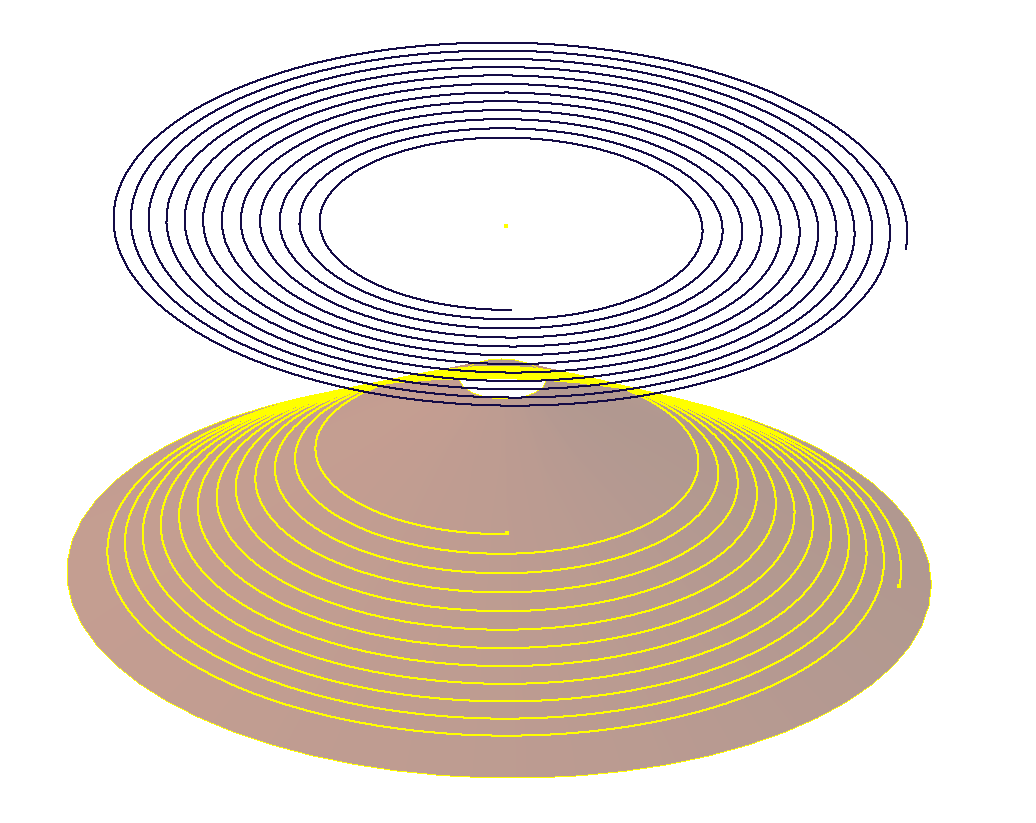
\includegraphics[width=0.9\textwidth]{kassandra/resources/JerJerWoBistDuSpirae.PNG}
    \caption{Projected Curve for the Bending Device}
    \label{fig:spirae}
\end{marginfigure}

\begin{figure}[h!]
    \centering
    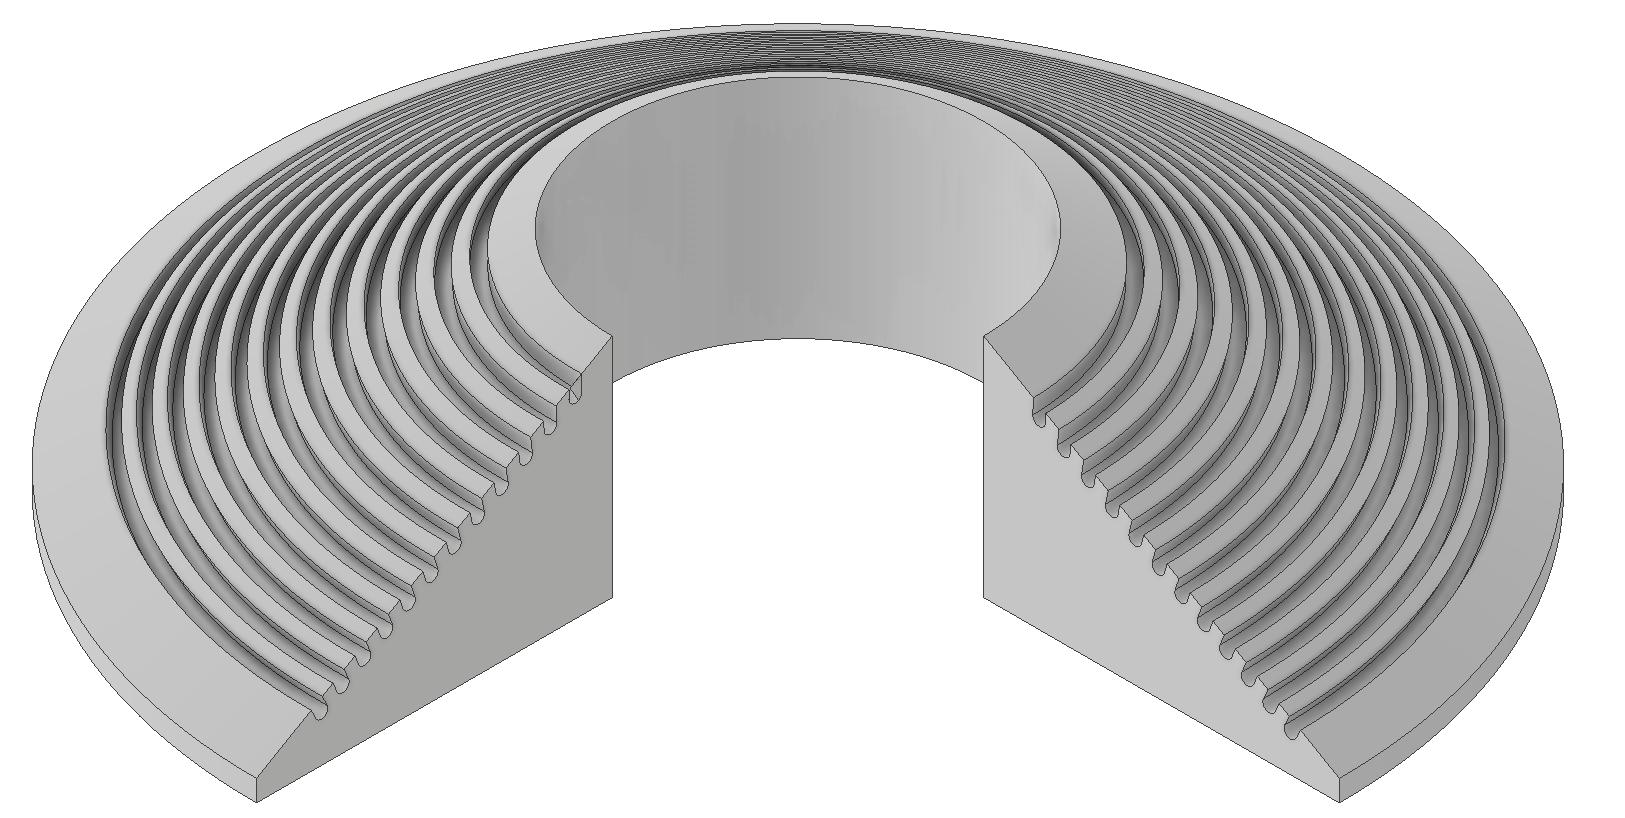
\includegraphics[width=0.7\textwidth]{kassandra/resources/JerJerWoBistDuBiegeBieg.PNG}
    \caption{Bending Device}
    \label{fig:biegbieg}
\end{figure}

\section{Top Electrode}

The top electrode needs to be made out of a temperature resistant, conductive material. It should already be available as thin rod, because turning would not be an option for such small diameters. Welding electrodes fit this criteria, because they are a few millimeters thick and consist of a tungsten alloy with a melting point of around \texttt{insert correct value here}. By using a bench grinder, one side of the electrode could easily be whetted to a pointy spike.

The holder that keeps the electrode at the top of the coil is made of two parts. As seen in figure \ref{fig:top-electrode}, the first is two copper pieces that are kept together with a thread, and in between, the wire of the secondary gets clamped. There are also two notches on each to enable fastening and opening with a flat wrench. To mount the tungsten electrode, a press fit was drilled into the top surface of the copper piece. The second part is a \gls{pmma} piece with another fit at the top for the copper piece. There is also a gap on one side to direct the wire of the secondary to the inner part. 

\begin{marginfigure}[-8cm]
    \centering
    \includegraphics[width=0.7\textwidth]{kassandra/resources/endeMeinerHoffnungFürBlitz.PNG}
    \caption{Mounting of the top electrode}
    \label{fig:top-electrode}
\end{marginfigure}

\subsection{It's not a Bug, it's a Feature}

Because the Tesla coil driver was very underdesigned, the plasma flame forming on the top electrode was very small and often had to be ignited and stabilized by another conductor held close to it. This was realized by placing a second, ancillary electrode over to the main electrode. This ancillary electrode is held by a canopy-like structure, resting on three \gls{pmma} rods. It was press fitted into a flat copper cylinder, which was loosely screwed into the cap. This way, its height and the gap between the two electrodes could be changed by turning the ancillary electrode. 

\begin{marginfigure}[-3cm]
    \centering
    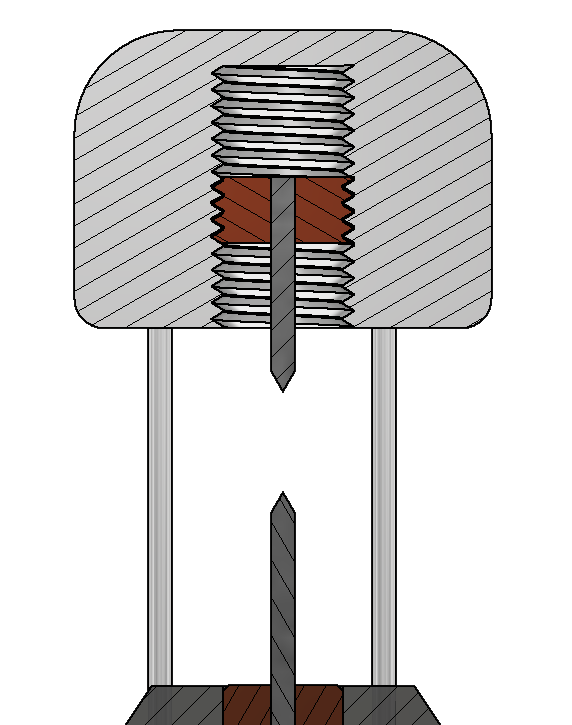
\includegraphics[width=\textwidth]{kassandra/resources/mirGehtsSuperDanke.png}
    \caption{Mounting of the ancillary electrode}
    \label{fig:ancillary-electrode}
\end{marginfigure}

To further examine the effect of the material of the cap, three different versions have been made. One out of \gls{pmma} and two out of Aluminium, one of which is as smooth as possible and one as pointy as possible.

\begin{figure}[h!]
    \centering
    \label{fig:caps}
    \begin{subfigure}[b]{0.4\textwidth}
        \centering
        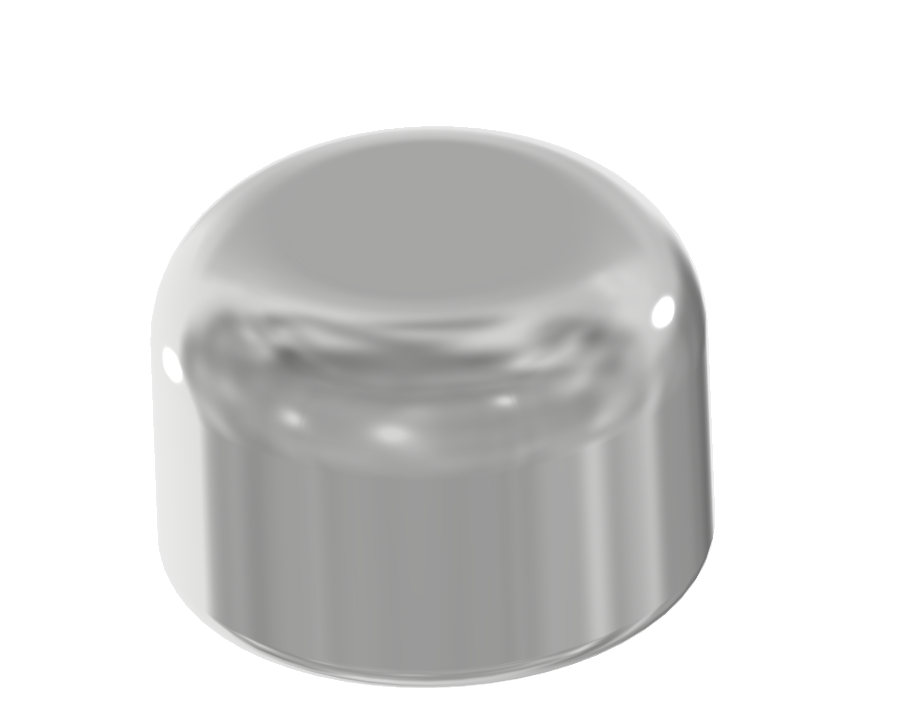
\includegraphics[width=0.9\textwidth]{kassandra/resources/mirGehtsSuperDankeSmooth.png}
    \end{subfigure}
    \hfill
    \begin{subfigure}[b]{0.4\textwidth}
        \centering
        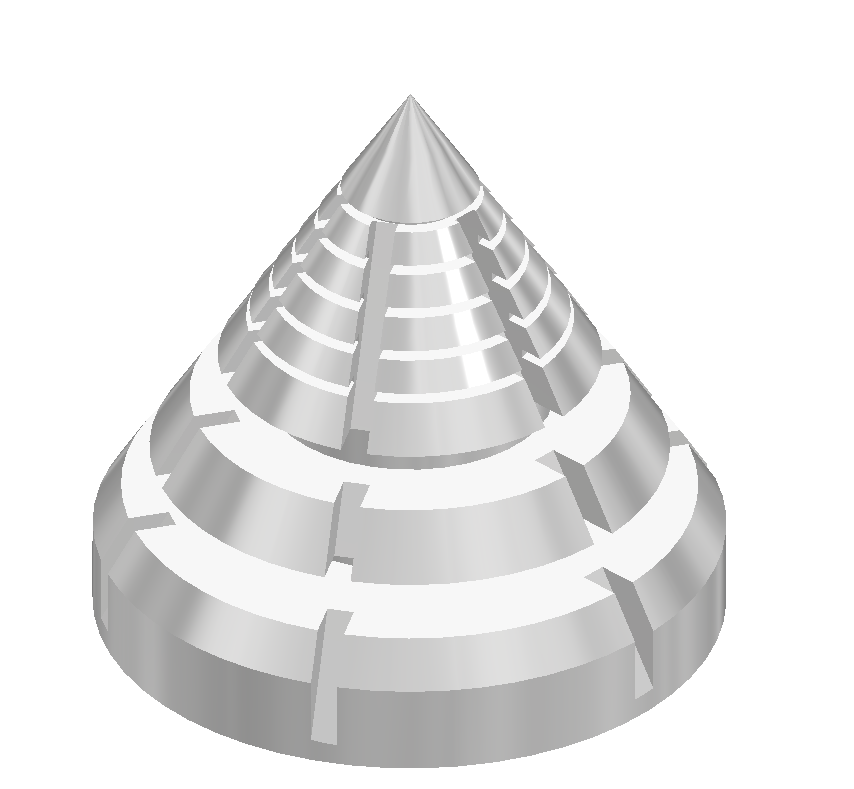
\includegraphics[width=0.9\textwidth]{kassandra/resources/mirGehtsSuperDankeEdgy.png}
    \end{subfigure}
    \caption{Smooth and Pointy Cap}
\end{figure}

While in section \ref{subsec:materials-metals}, it was explained that metals pose a safety hazard, this is not entirely true for the secondary side of the Tesla coil. Despite the high voltages of up to several kilovolts present at the top electrode, it is relatively safe to touch. This is because as soon as a low-resistance path to ground, like a human, opens for the current, the voltage drops to a very low level, which means that the resulting current cannot do any harm besides the usual burned skin.

\section{PCB Enclosure}

The general placement of the \gls{pcb}, being right beneath the coils, was already addressed in section \ref{sec:concept-design}. The platform where the secondary coil and the supports for the primary coil are mounted was already designed and chosen to be hexagon-shaped, mainly because it works the best with the six supports. Again, the prototype has the platform resting on top of six pillars to keep everything as modular as possible. The prototype also has only the most essential features and only consists of a framework, this also makes it easier to access the inside of the \gls{pcb} enclosure. The final design would be completely closed off, and the platform would be glued on as like the primary coil’s supports.

\begin{figure}[h!]
    \centering
    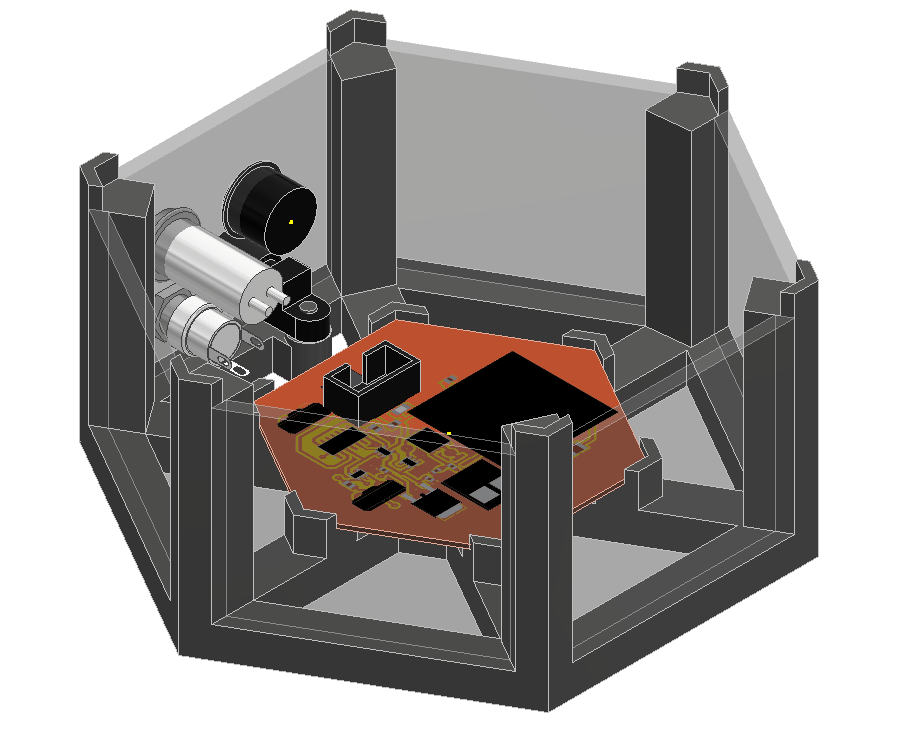
\includegraphics[width=0.9\textwidth]{kassandra/resources/JerJerWoBistDu.PNG}
    \caption{PCB Enclosure}
    \label{fig:bottom-bau}
\end{figure}

\subsection{PCB}

The hexagonal \gls{pcb} was placed in the center of the enclosure right under the secondary, mostly to balance the design. To ensure that the circuit can also give off heat on the bottom side, it cannot be mounted directly onto the enclosure and therefore has to be raised by a few millimeters. This is done by six steps onto which the \gls{pcb} is screwed. 

\begin{marginfigure}[-3cm]
    \centering
    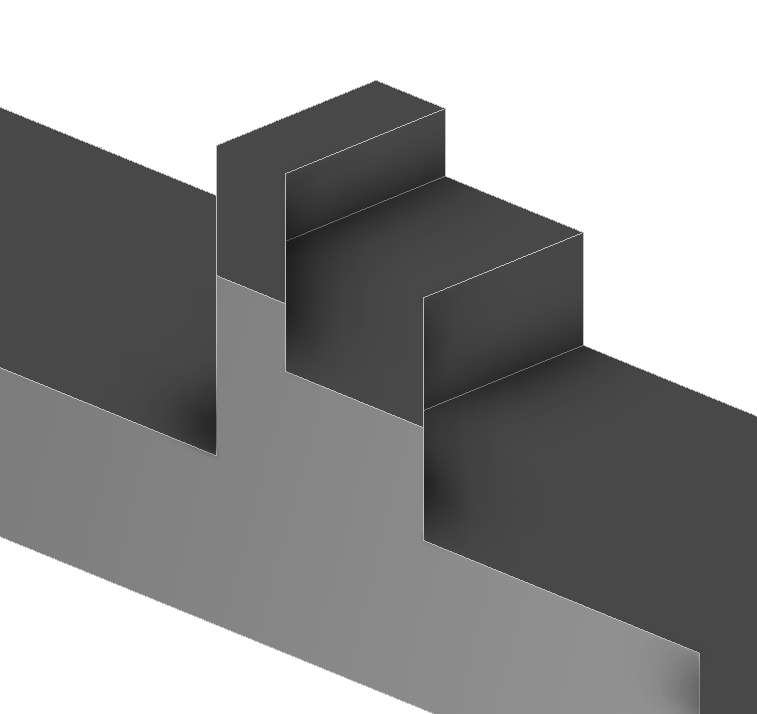
\includegraphics[width=0.7\textwidth]{kassandra/resources/JerJerWoBistDuStufe.PNG}
    \caption{PCB Holder}
    \label{fig:bottom_stufe}
\end{marginfigure}
    
